 %%	SECCION documentclass																									 %%	
%%---------------------------------------------------------------------------%%
\documentclass[a4paper]{report}

%%---------------------------------------------------------------------------%%
%%	SECCION usepackage																											 %%	
%%---------------------------------------------------------------------------%%
\usepackage{amsmath, amsthm}
\usepackage[spanish,activeacute]{babel}
\usepackage{caratula}
\usepackage{a4wide}
\usepackage{hyperref}
\usepackage{fancyhdr}
\usepackage{graphicx} % Para el logo magico!
\usepackage{amssymb}
\usepackage{amsmath}
\usepackage{float}
\usepackage[latin1]{inputenc}
%\usepackage [T1]{fontenc}
\usepackage[dvipsnames,usenames]{color}
\usepackage{amsfonts}
\usepackage{ulem}
%\usepackage{highlight}
\usepackage{fancybox}
%\usepackage{marvosym}
\usepackage{color}
\usepackage{lastpage}
\usepackage{lscape}
\usepackage{tabularx}
\usepackage{algorithmic}
\usepackage{algorithm}
\usepackage{subfigure}

%%---------------------------------------------------------------------------%%
%%	SECCION opciones																												 %%	
%%---------------------------------------------------------------------------%%
\parskip    = 11 pt
\headheight	= 13.1pt
\pagestyle	{fancy}
\definecolor{orange}{rgb}{1,0.5,0}

\addtolength{\headwidth}{1.0in}

\addtolength{\oddsidemargin}{-0.5in}
\addtolength{\textwidth}{1.0in}
\addtolength{\topmargin}{-0.5in}
\addtolength{\textheight}{0.7in}

%%---------------------------------------------------------------------------%%
%%	SECCION document	 %%	
%%---------------------------------------------------------------------------%%
\begin{document}
\renewcommand{\chaptername}{Parte }
\renewcommand{\algorithmicrequire}{\textcolor{blue}{\textbf{Requiere:}}}
\renewcommand{\algorithmicensure}{\textbf{Asegura:}}
\renewcommand{\algorithmicend}{\textbf{Fin}}
\renewcommand{\algorithmicif}{\textcolor{blue}{\textbf{Si}}}
\renewcommand{\algorithmicthen}{\textcolor{blue}{\textbf{entonces}}}
\renewcommand{\algorithmicelse}{\textcolor{red}{\textbf{Si no}}}
\renewcommand{\algorithmicelsif }{\textcolor{blue}{\textbf{Si no y}}}
\renewcommand{\algorithmicendif}{\textcolor{blue}{\textbf{Fin si}}}
\renewcommand{\algorithmicfor}{\textcolor{ForestGreen}{\textbf{Para}}}
\renewcommand{\algorithmicendfor}{\textcolor{ForestGreen}{\textbf{Fin para}}}
\renewcommand{\algorithmicwhile}{\textcolor{ForestGreen}{\textbf{Mientras}}}
\renewcommand{\algorithmicendwhile}{\textcolor{ForestGreen}{\textbf{Fin mientras}}}
\renewcommand{\algorithmicdo}{\textcolor{ForestGreen}{\textbf{hacer}}}
\renewcommand{\algorithmicreturn}{\textbf{Devolver}}
\floatname{algorithm}{Algoritmo}

%%---- Caratula -------------------------------------------------------------%%
\materia{Investigaci�n Operativa (2do cuatrimestre de 2010)}
\titulo{Trabajo Pr�ctico}

\integrante{Gonzalez, Emiliano}{426/06}{xjesse\_jamesx@hotmail.com}
\integrante{Gonzalez, Sergio}{481/06}{gonzalezsergio2003@yahoo.com.ar}
\resumen{
En el siguiente documento, se mostrar�n diferentes pruebas de performance utilizando la herramienta CPLEX. Las pruebas consisten en la modificaci�n de diferentes t�cnicas de brancheo del m�todo Branch and Bound y del m�todo Branch and Cut, esta �ltima con una parte implementada especialmente para resolver el problema de separaci�n.}

% TOC, usa estilos locos
\maketitle
\pagestyle{empty}
{
\fancypagestyle{plain}
    {
    \fancyhead{}
    \fancyfoot{}
    \renewcommand{\headrulewidth}{0.0pt}
    } % clear header and footer of plain page because of ToC
\tableofcontents
}

\newpage
% arreglos los estilos para el resto del documento, y
% reseteo los numeros de pagina para que queden bien
\pagenumbering{arabic}
\fancypagestyle{plain} {
    \fancyhead[LO]{Gonzalez, Gonzalez, Tleye}
    \fancyhead[C]{}
    \fancyhead[RO]{P\'agina \thepage\ de \pageref{LastPage}}
    \fancyfoot{}
    \renewcommand{\headrulewidth}{0.4pt}
}
\pagestyle{plain}

%\newpage
%\section{Ejercicio1}

El objetivo de este ejercicio consiste en poner a prueba el problema de coloreo, variando algunos de los par�metros que $Cplex$ utiliza para resolver el problema. Los mismos son par�metros gen�ricos que forman parte del comportamiento que tiene $Cplex$ para computar la soluci�n.

En este caso en particular, se tomaron par�metros que se utilizan en el m�todo de Branch and Bound. La prueba entonces, consiste en modificar los valores de dichos par�metros y observar como es el desempe�o del proceso, en tiempo requerido y en cantidad de nodos creados por $Cplex$, hasta obtener la soluci�n del problema.

Los par�metros elegidos son los siguientes:

\begin{itemize}
\item \textbf{CPX\_PARAM\_BRDIR:} Este par�metro sirve para modificar la direcci�n en la cual se har� en branching en cada paso. Los posibles valores para el mismo son los siguientes:
   \begin{itemize}
   \item CPX\_BRDIR\_UP, que indica que el branching siempre debe hacerse por la parte superior.
   \item CPX\_BRDIR\_DOWN, que indica que el branching debe hacerse por la parte inferior.
   \item CPX\_BRDIR\_AUTO, que indica que $Cplex$ decidir� que camino tomar.
   \end{itemize}

\item \textbf{CPX\_PARAM\_LBHEUR:} Indica si las heur�sticas locales en cada branching est�n o no activadas. Los valores para el mismo son: CPX\_ON y CPX\_OFF.

\item \textbf{CPX\_PARAM\_VARSEL:} CPX\_PARAM\_LBHEUR depende de este par�metro, que indica que estrategia usar para seleccionar una variable antes de realizar el branching. Los posibles valores son:
    \begin{itemize}
    \item CPX\_VARSEL\_MININFEAS, que realiza el branch con la variable con inviabilidad m�nima (es decir, la variable fraccionaria mas cercana a alg�n valor entero).
    \item CPX\_VARSEL\_MAXINFEAS, que realiza el braching con la variable mas inviable(es decir la mas lejana a un valor entero)
    \item CPX\_VARSEL\_PSEUDO, la variable es elegida a trav�s de pseudo costos.
    \item CPX\_VARSEL\_PSEUDO, elije la variable a trav�s de la resoluci�n de diferentes sub problemas que permiten saber cuan prometedora es la elecci�n de dicha variable.
    \item CPX\_VARSEL\_PSEUDOREDUCED, selecciona la variable basado en costos.
    \end{itemize}

\item \textbf{CPX\_PARAM\_STRONGITLIM:} Indica el l�mite de iteraciones a realizar en cada una de las variables candidatas para realizar el branching. Los valores que puede tomar son: 0, automatico o un n�mero positivo, que indica las iteraciones fijas a realizar.

\item \textbf{CPX\_PARAM\_ZEROHALFCUTS:} Aqu� se indica si se har�n o no cortes de tipo parte entera hacia abajo para los valores de algunas de las restricciones. Los posibles valores son: -1, desactivado, 0 automatico, 1 normal y 2 agresivo.
\end{itemize}

\subsection{Pruebas realizadas}


%\clearpage

\newpage
\section{Ejercicio 2}

Para demostrar que las desigualdades son v�lidas, se utilizar� el m�todo del absurdo. La desigualdad es v�lida para el $CP$ original (sin relajaci�n) si la desigualdad se cumple para todos los puntos dentro de la c�psula convexa de soluciones factibles enteras. Por lo tanto el planteo inicial ser� suponer que el punto no cumple con la nueva restricci�n pero s� con las condiciones originales.

Supongamos que existe un coloreo v�lido para el $CP$ original. Por lo tanto existe $W$ = $(w_0, w_1, ... , w_n)$ y $X = \{x_{vj} | v = 0, ..., n \wedge j = 0, ..., n\}$, donde $v$ son los nodos y $j$ son los colores con los que se pintaron los mismos. Entonces para $X$ vale:

\begin{enumerate}
\item $\displaystyle\sum_{j = 1}^{n} x_{pj} = 1$, $\forall$ $p \in V$

\item $x_{pj} + x_{qj} \le w_j$, $\forall$ $(p,q) \in E$, $j = 1,...,n$

\item $x_{pj} \in \{0,1\}$, $\forall$ $p \in V$, $j = 1,...,n$

\item $w_j \in \{0,1\}$, $\forall$ $j = 1,...,n$

\end{enumerate}

\subsection{Desigualdad 1: Clique}

Sea K una Clique del grafo y sea $j_0$ cualquier color tal que $1 \le j_0 \le n$. Supongamos que la soluci�n no cumple con la desigualdad clique, entonces sabemos que vale lo siguiente:

$$\displaystyle\sum_{p \in K} x_{pj_0} > w_{j_0}$$

\begin{itemize}

\item Supongamos que $|K| = 2$. Sean dos nodos cualesquiera $p_1$ y $p_2$ de la Clique, entonces vale que:

$$x_{{p_1}{j_0}} + x_{{p_2}{j_0}} > w_{j_0}$$

Pero por otro lado, como K es una clique, sabemos que existe un eje $({p_1},{p_2})$ de modo que se cumple la condici�n (2) del $CP$ original:

$$x_{{p_1}{j_0}} + x_{{p_2}{j_0}} \le w_{j_0}$$

Pero esto resulta ser absurdo ya que no puede pasar que $A > w_{j_0}$ y que $A \le w_{j_0}$ siendo $A = x_{{p_1}{j_0}} + x_{{p_2}{j_0}}$.$\qed$


\item Supongamos ahora que $|K| > 2$. Sean tres nodos cualesquiera $p_1$, $p_2$ y $p_3$ de la Clique, entonces vale que:

$$x_{{p_1}{j_0}} + x_{{p_2}{j_0}} + x_{{p_3}{j_0}} + ... + x_{{p_n}{j_0}} > w_{j_0}$$

Por otro lado, como K es una clique, sabemos que existen ejes $({p_1},{p_2})$, $({p_2},{p_3})$, $({p_3},{p_1})$ de modo que se cumplen las condiciones (2) del $CP$ original:

$$x_{{p_1}{j_0}} + x_{{p_2}{j_0}} \le w_{j_0}$$

$$x_{{p_2}{j_0}} + x_{{p_3}{j_0}} \le w_{j_0}$$

$$x_{{p_3}{j_0}} + x_{{p_1}{j_0}} \le w_{j_0}$$

\medskip
Entonces vale decir lo siguiente:

$$x_{{p_1}{j_0}} + x_{{p_2}{j_0}} \le w_{j_0} < x_{{p_1}{j_0}} + x_{{p_2}{j_0}} + x_{{p_3}{j_0}} + ... + x_{{p_n}{j_0}}$$

Por lo tanto se deduce lo siguiente:

$$x_{{p_3}{j_0}} + ... + x_{{p_n}{j_0}} > 0$$

Podemos suponer, sin p�rdida de generalidad, que $x_{{p_3}{j_0}} = 1$.

\medskip
Por otro lado tenemos que:

$$x_{{p_2}{j_0}} + x_{{p_3}{j_0}} \le w_{j_0}$$

Por condici�n (2) del $LP$ original. Entonces vale lo siguiente:

$$x_{{p_2}{j_0}} + x_{{p_3}{j_0}} \le w_{j_0} < x_{{p_1}{j_0}} + x_{{p_2}{j_0}} + x_{{p_3}{j_0}} + ... + x_{{p_n}{j_0}}$$

Por lo tanto:

$$x_{{p_1}{j_0}} + x_{{p_4}{j_0}} + ... + x_{{p_n}{j_0}} > 0$$

Nuevamente, sin p�rdida de generalidad suponemos que $x_{{p_1}{j_0}} = 1$. Pero se sab�a por lo anterior que:

$$x_{{p_3}{j_0}} + x_{{p_1}{j_0}} \le w_{j_0}$$

Por lo tanto, se llega a que:

$$w_{j_0} \geq 2$$

Lo cual resulta absurdo, pues por (4) $w_j \in \{0, 1\} \forall 1 \le j \le n$. $\qed$

\end{itemize}

Dado que no hay m�s alternativas, la suposici�n de que la desigualdad no se cumple es falsa. $\qed$

\subsection{Desigualdad 2: Agujero de Longitud Impar}

Sea $C_{2k+1}$ el conjunto de v�rtices dentro de un agujero de longitud $2k+1$, con $k >= 2$. Supongamos que la soluci�n no cumple con la desigualdad agujero impar. Por lo tanto podemos decir que $\exists k >= 2$ tal que:

$$
\sum_{p \in C_{2k+1}} x_{p{j_0}} > kw_{j_0}
$$

Con $j_0$ cualquier color tal que $1 \le j_0 \le n$.

\begin{itemize}
\item Supongamos que $w_{j_0} = 0$. Para este caso la desigualdad quedar�a de la siguiente forma:

$$
\sum_{p \in C_{2k+1}} x_{p{j_0}} > 0
$$
      
Como se puede observar, la restricci�n se cumple si existe alg�n nodo $p$ del agujero $C_{2k+1}$ tal que $x_{p{j_0}} = 1$. Dado que no hay nodos aislados, podemos tomar un eje $(p,p')$ de modo que se cumple la condici�n (2) del $CP$ original:

$$x_{{p}{j_0}} + x_{{p'}{j_0}} \le w_{j_0}$$

O sea que

$$x_{{p'}{j_0}} + 1 \le w_{j_0}$$

Pero por (3) $x_{{p'}{j_0}} \in \{0,1\}$, y $w_{j_0} = 0$, o sea que $x_{{p'}{j_0}} + 1 \le 0$ lo cual es absurdo. $\qed$

\item Supongamos ahora que $w_{j_0} = 1$. Para este caso la desigualdad quedar�a de la siguiente forma:

$$
\sum_{p \in C_{2k+1}} x_{p{j_0}} > k
$$
      
La restricci�n entonces se cumple si hay almenos $k+1$ nodos del agujero pintados con el color $j_0$.

Para un circuito de longitud $2k+1$, la m�xima cantidad de nodos pintados del mismo color para que su coloreo sea v�lido es $k$. Como los nodos del agujero conforman un circuito de longitud impar, si pintamos $k+1$ o m�s nodos del mismo color, este coloreo ser�a inv�lido para el mismo circuito, por lo tanto hay almenos dos nodos que son adyacentes entre s� y est�n pintados del mismo color. Por consiguiente el coloreo es inv�lido y la suposici�n de que $w_{j_0} = 1$ es absurda. $\qed$

\end{itemize}

Dado que no hay m�s alternativas, la suposici�n de que la desigualdad no se cumple es falsa. $\qed$

\clearpage

%\newpage
%\section{Ejercicio 3}

%TODO:hacerlo

%\clearpage

%\newpage
%\section{Ejercicio 4}

En esta secci�n se har�n comparaciones entre los algoritmos de las secciones anteriores con un algoritmo que corre $CPLEX$ standard con los par�metros por defecto. Adem�s, se analizar� c�mo aportan nuestras heur�sticas y algoritmos de separaci�n a $CPLEX$ por defecto.

Los an�lisis y las comparaciones se har�n en base a una serie de tipos de tests que tienen diferentes configuraciones entre los cortes a usar, las heur�sticas iniciales y diferentes par�metros que definen el comportamiento del Branching. Los tipos de test, son los siguientes:

\begin{enumerate}
\item Tipo 1: Se setean las heur�sticas iniciales propias, sin activar las heur�sticas iniciales de $CPLEX$. Se desactivan todos los tipos de cortes. Se setean los par�metros de Branching seg�n el tipo 7 de los tipos del ejercicio n�mero 1.

\item Tipo 2: Se setean las heur�sticas iniciales propias, sin activar las de $CPLEX$. Se activan los cortes de $CPLEX$ (sin los cortes Clique y Agujero Impar implementados). Se setean los par�metros de Branching seg�n el tipo 7 de los tipos del ejercicio n�mero 1.

\item Tipo 3: Se setean las heur�sticas iniciales propias, sin activar las de $CPLEX$. Se activan los cortes de $CPLEX$ y los cortes Clique y Agujero Impar implementados. Se setean los par�metros de Branching seg�n el tipo 7 de los tipos del ejercicio n�mero 1.

\item Tipo 4: Se setean las heur�sticas iniciales propias, sin activar las de $CPLEX$. Se activan los cortes de $CPLEX$ y los cortes Clique y Agujero Impar implementados. Se setean los par�metros de Branching de forma autom�tica, dejando que $CPLEX$ elija el apropiado seg�n el caso.

\item Tipo 5: Solo $CPLEX$. Se setean las heur�sticas iniciales y cortes de $CPLEX$. Se setean los par�metros de Branching de forma autom�tica, dejando que $CPLEX$ elija el apropiado seg�n el caso.

\end{enumerate}

Con estos tipos de tests, se espera ver como se comportan las heur�sticas implementadas versus las heur�sticas iniciales de $Cplex$, el rendimiento en tiempo y cantidad de nodos entre $Cplex$ autom�tico versus las variantes que se ten�an en secciones anteriores.

A continuaci�n se describir�n cuales son las instancias con las cuales se har�n las pruebas para cada tipo:

\begin{enumerate}
\item test 1: La primera de las instancias es el grafo myciel4, que es un grafo libre de tri�ngulos y con 23 nodos.

\item test 2: Grafo generado aleatoriamente, con una cantidad de 42 nodos y una densidad de 25\%.

\item test 3: Grafo generado aleatoriamente, con una cantidad de 42 nodos y una densidad de 50\%.

\item test 4: Grafo generado aleatoriamente, con una cantidad de 42 nodos y una densidad de 75\%.

\item test 5: Grafo generado aleatoriamente, con una cantidad de 45 nodos y una densidad de 25\%.

\item test 6: Grafo generado aleatoriamente, con una cantidad de 45 nodos y una densidad de 50\%.

\item test 7: Grafo generado aleatoriamente, con una cantidad de 45 nodos y una densidad de 75\%.

\item test 8: La �ltima instancia es el grafo myciel5, que es un grafo libre de tri�ngulos y con 47 nodos.

\end{enumerate}

\subsection{Resultados}

\begin{figure}[H]
\centering
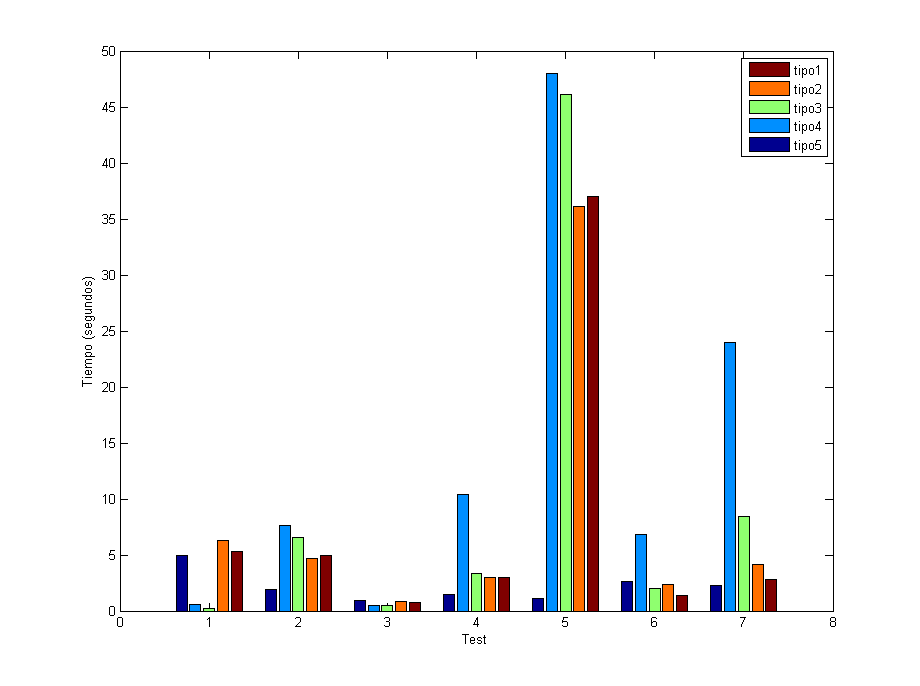
\includegraphics[scale=0.7]{../tests/resultados/resultados5/graficoTiemposEj4Tp.png}
\caption{Tiempo en segundos para cada test}
\end{figure}

En este gr�fico se puede observar que $CPLEX$ configurado en todo autom�tico generalmente prevalece en tiempos. Esto puede ser debido a que los cortes implementados no son del todo performantes o que $CPLEX$ se configura bien autom�ticamente. De todos modos los tiempos de ejecuci�n se pueden llegar a reducir si probamos con otras configuraciones de los par�metros de $CPLEX$.

\begin{figure}[H]
\centering
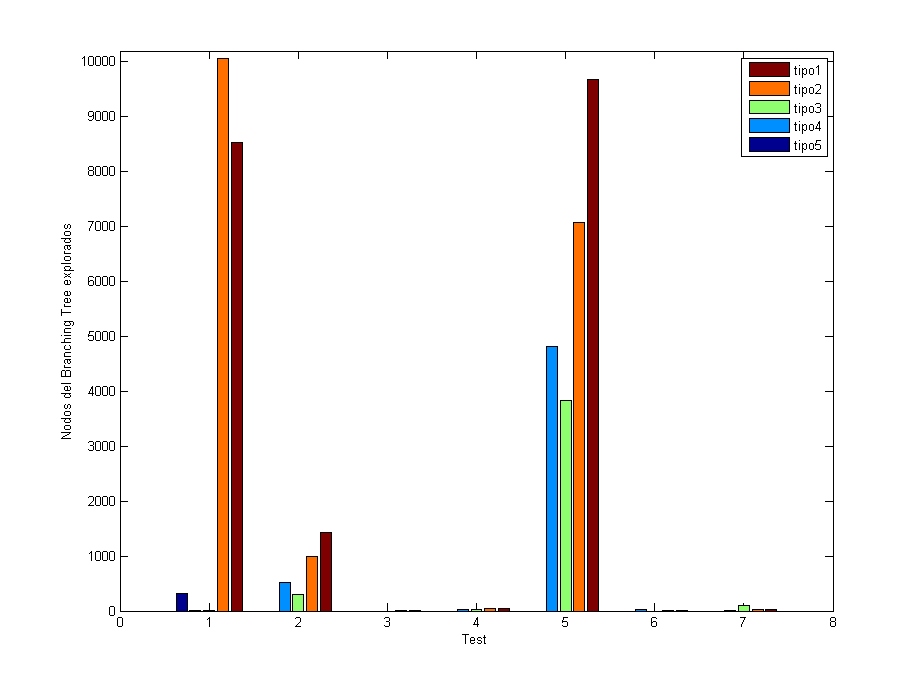
\includegraphics[scale=0.7]{../tests/resultados/resultados5/graficoNodosEj4Tp.png}
\caption{Nodos explorados del Branching Tree para cada test}
\end{figure}

En este gr�fico nuevamente se puede observar que $CPLEX$ configurado en todo autom�tico generalmente recorre menos nodos. Esto puede ser debido a que los cortes implementados no son del todo eficientes o que $CPLEX$ se configura bien autom�ticamente. Sin embargo puede notarse diferencias entre aquellos tests que utilizan los cortes implementados y aquellos que no, pues por lo general estos �ltimos recorren mayor cantidad de nodos que los primeros.

\begin{figure}[H]
\centering
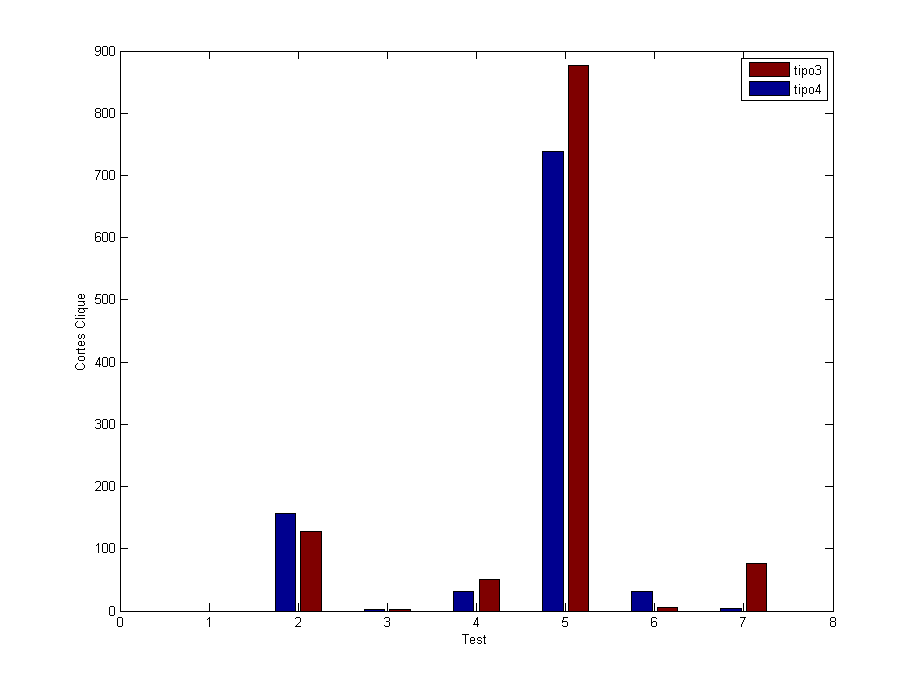
\includegraphics[scale=0.7]{../tests/resultados/resultados5/graficoCortesCliqueEj4Tp.png}
\caption{Cortes Clique para cada test}
\end{figure}

En este gr�fico se compara la cantidad de cortes Clique (de los implementados) hechos en cada caso de test que los tenga activados. Por razones obvias no se incluyen los otros tipos de test en la comparaci�n. Se puede confirmar que se logra hacer un gran aporte a $CPLEX$ en cuanto a la cantidad de cortes en cada nodo del Branching Tree. Es por esto que anteriormente en el gr�fico de la cantidad de nodos explorados ve�amos una diferencia entre aquellos tipos de test que usaban los cortes y aquellos que no.

\begin{figure}[H]
\centering
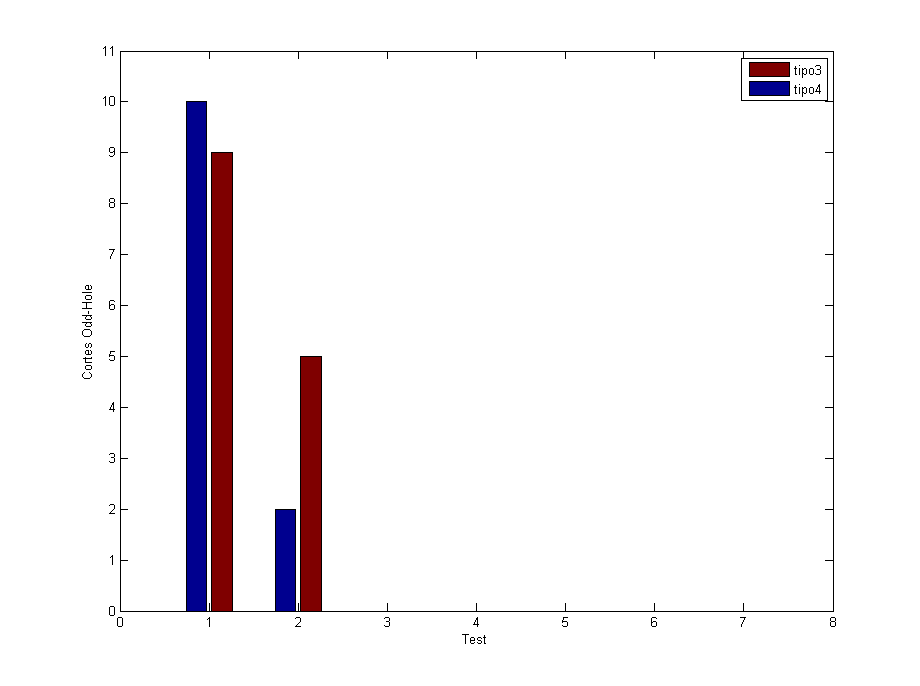
\includegraphics[scale=0.7]{../tests/resultados/resultados5/graficoCortesOddHoleEj4Tp.png}
\caption{Cortes Odd-Hole para cada test}
\end{figure}

En este gr�fico se compara la cantidad de cortes Odd-Hole (de los implementados) hechos en cada caso de test que los tenga activados. Por razones obvias no se incluyen los otros tipos de test en la comparaci�n. Como se ve este tipo de cortes no hace gran aporte a $CPLEX$, pero pudimos confirmar que el mismo es muy eficiente para por lo menos una cierta clase de grafos: aquellos tal que su clique m�xima es de 2 (dos) nodos. Se ejecutaron los mismos tipos de test para el test 8 (myciel5) y se logra una excelente performance:
\[
\begin{array}{cccc}
	tiempo(segundos)	&	Odd-Hole	&	Clique	&	nodos\\
	\hline
	19.782	&	254 & 0 & 772 \\
	23.953	&	221 & 0 & 849 \\
\end{array}
\]

Los test de tipo 1, 2 y 5 que son los que tienen los cortes desactivados tardan un tiempo significativamente mayor (m�s que 20 minutos).

Hubieron much�simos tests generados al azar (de hasta 80 nodos) que no tardaron en resolverse gracias a que las heur�sticas iniciales daban igual cota inferior que superior, por lo que la funci�n objetivo quedaba vac�a. Sin embargo estos tests no fueron inclu�dos en este informe debido a que no aportaban informaci�n alguna para este an�lisis.
%\clearpage

\label{LastPage}
\end{document}
